%TCIDATA{LaTeXparent=0,0,relatorio.tex}

\chapter{Errata}

\paragraph{Conclusão} O capítulo de conclusão deveria incluir uma seção de propostas de projetos implementáveis ou otimizáveis através da autorreconfiguração.
Seguem a seguir as modificações necessárias.

\section{Propostas de Aplicações}
O objetivo deste projeto deste o início foi o desenvolvimento de um sistema capaz de realização de autorreconfiguração, o que consitui o ápice tecnológico da reconfiguração dinâmica parcial.
Tendo-se compreendido o fluxo de desenvolvimento para o uso desta tecnologia, propõe-se agora algumas possíveis aplicações.

\subsection{Redes Neurais}
\paragraph{Introdu\c{c}\~ao}
Redes neurais s\~ao uma ferramenta de inteligência artificial largamente utilizada nas \'areas de \textit{Data Mining} e sistemas que necessitem de algum tipo de aprendizado.
Elas utilizam de redes de elementos extremamente simples, como mostrado na figura \ref{fig:nn}, para criar uma fun\c{c}\~ao altamente n\~ao-linear com um comportamento esperado.
Estes elementos podem ser matematicamente representados por somat\'orios ponderados afunilados por fun\c{c}\~oes n\~ao-lineares.
Os pesos utilizados nestes somat\'orios s\~ao os elementos a serem adaptados de forma a modificar o comportamento da estrutura.
Elas podem ser utilizadas tanto aprendizados supervisionados, onde funciona como um poderoso aproximador de fun\c{c}\~oes, quanto em aprendizados n\~ao-supervisionados, onde traduz um sistema hiperdimensional em bidimensional.

\begin{figure}[h]
\centering
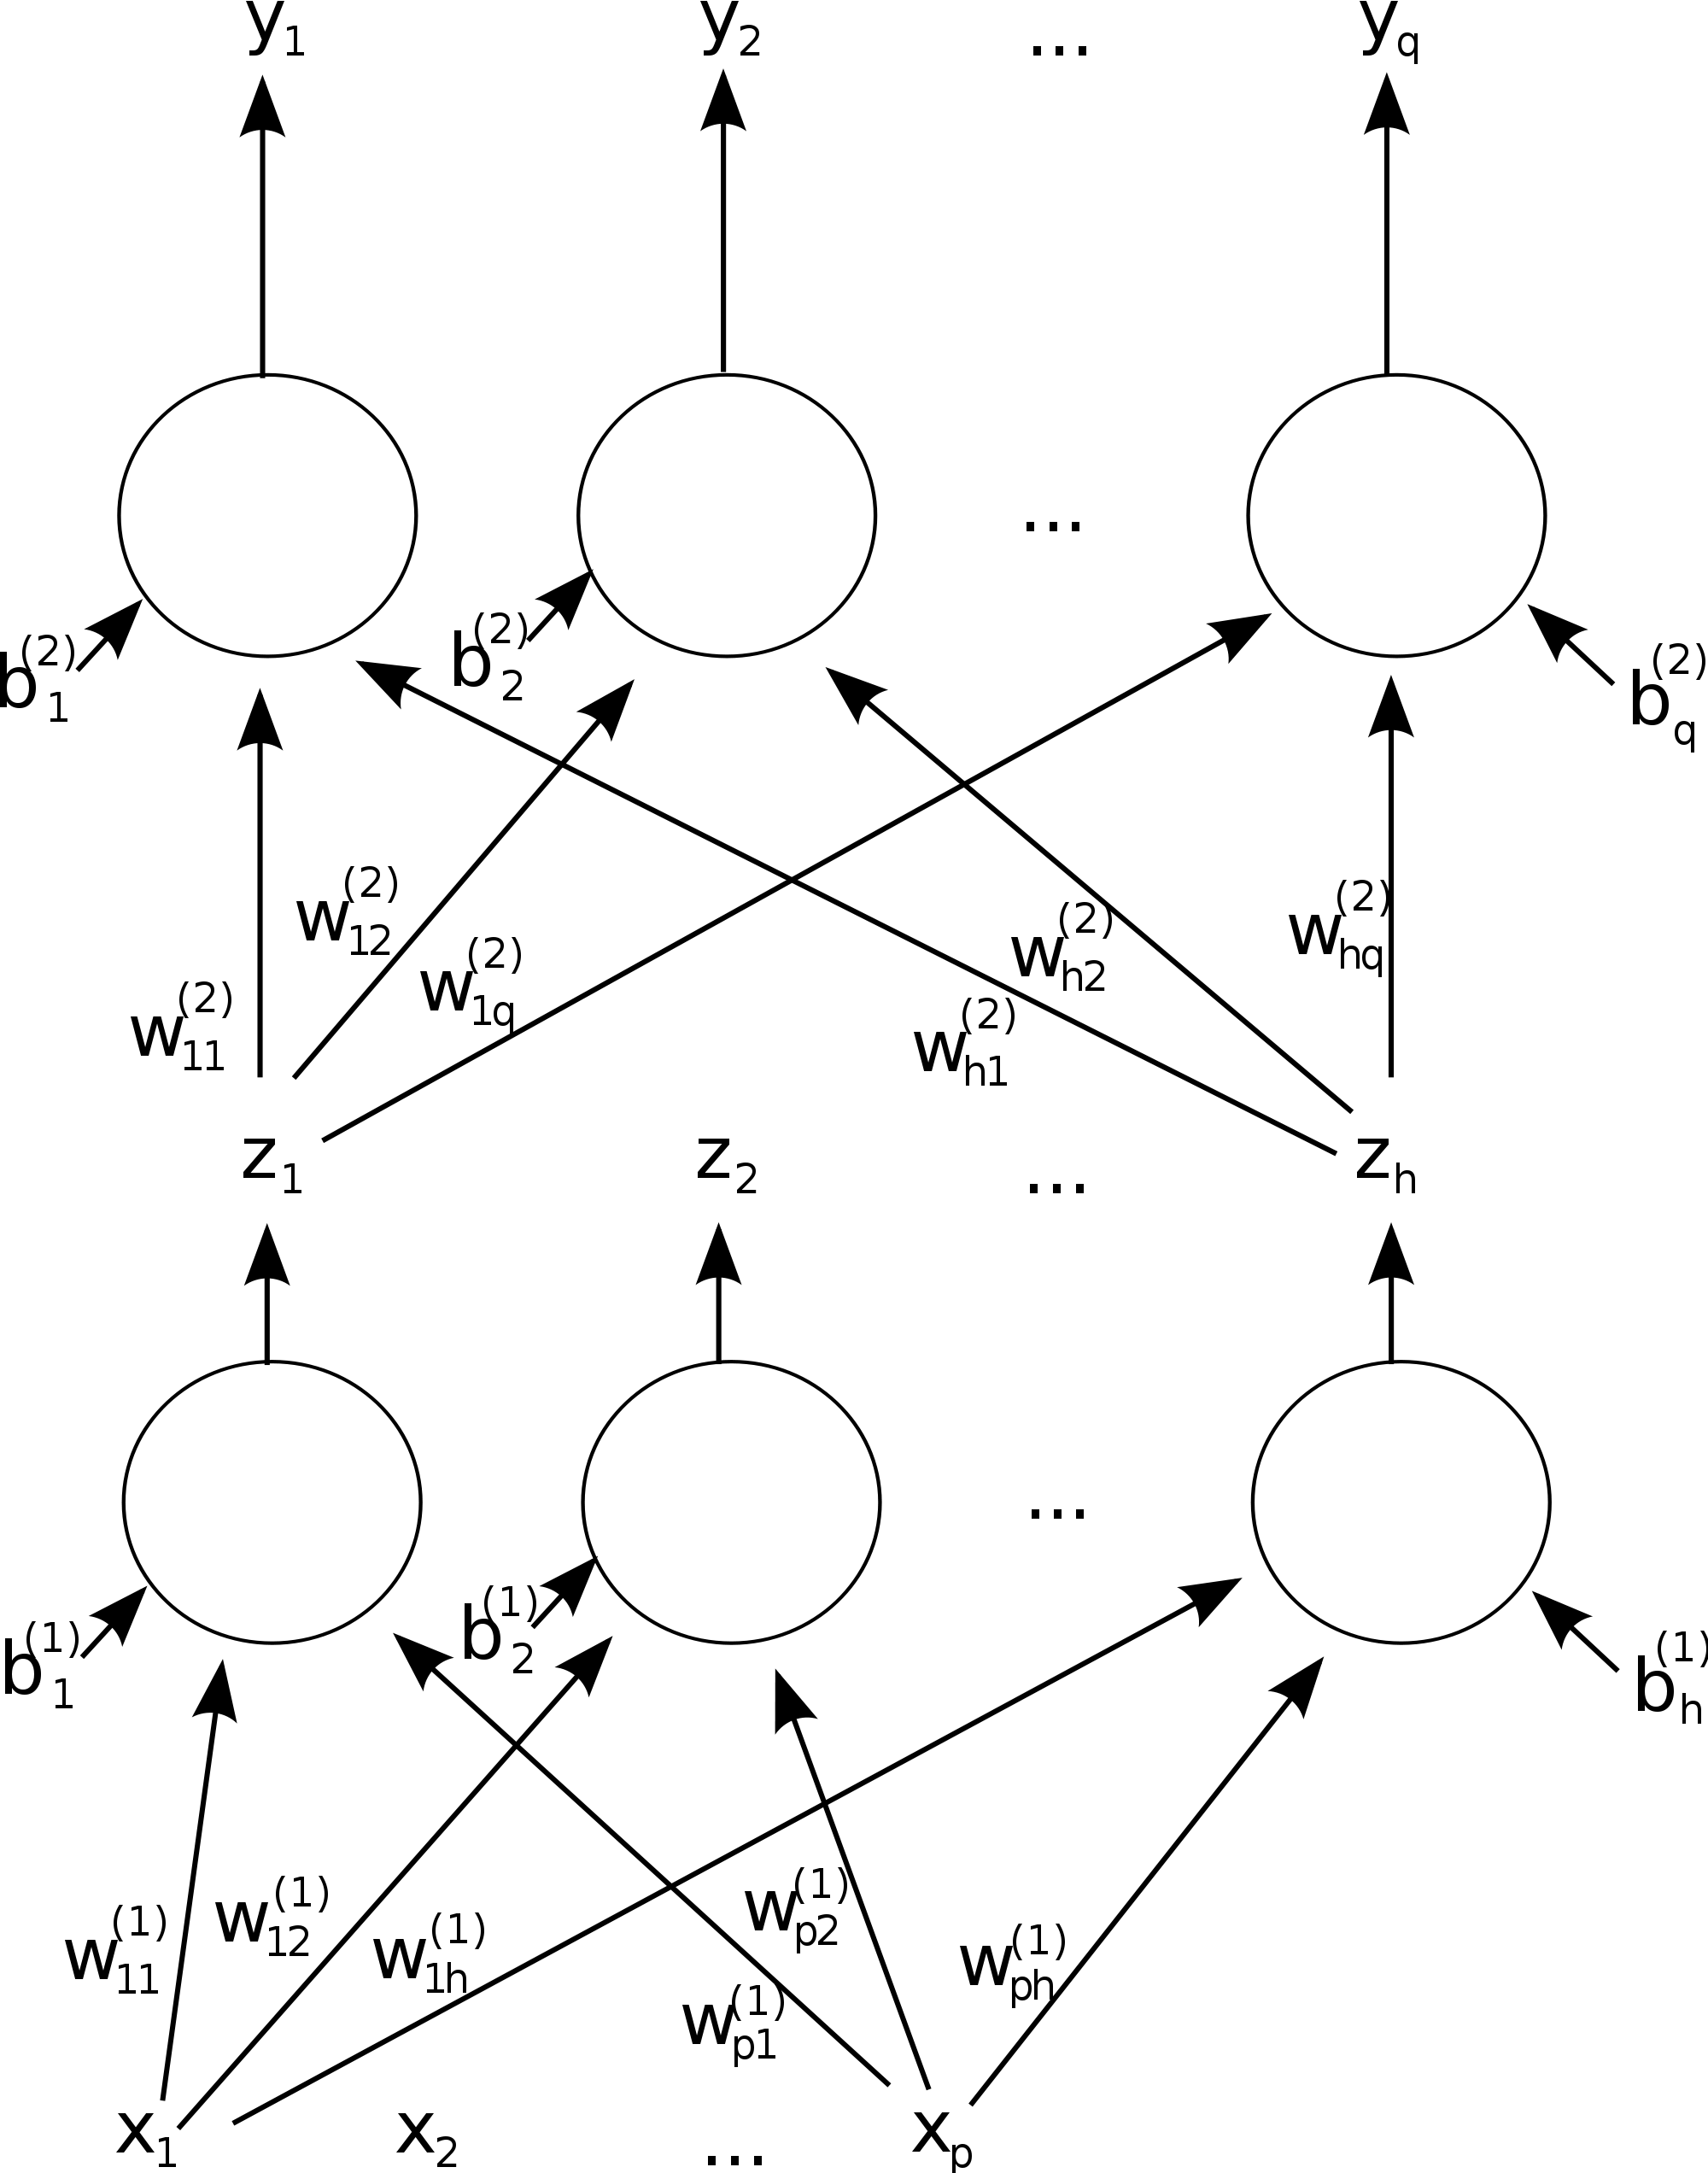
\includegraphics[width=0.5\textwidth]{fig/propostas/model_nn}
\caption{Modelo de rede neural com "$p$" entradas, "$q$" saídas e duas camadas.}
\label{fig:nn}
\end{figure}

\paragraph{Topologias}
As redes neurais podem possuir v\'arias camadas de neur\^onios, que s\~ao as unidades b\'asicas de processamento, e v\'arias entradas e saídas.
Quanto mais camadas s\~ao acrescentadas ao sistema, mais inst\'avel fica seu treinamento e custosa sua computa\c{c}\~ao.
Em geral utilizam-se apenas duas ou três camadas com um n\'umero arbitr\'ario de neur\^onios em cada uma.
N\~ao existe um algoritmo que determine qual seria a topologia ideal de uma rede para um certo modelo.
Tal decis\~ao normalmente \'e feita com base em experiência e tentativas e erros.

Existem topologias três topologias b\'asicas de redes neurais: a \textit{feedforward}, a recorrente e a atrasada.
A primeira possui neur\^onios que entregam seus resultados apenas para camadas mais a frente.
A segunda, mais complexa, al\'em de entregar seus resultados para as camadas mais a frente, realimentam camadas anteriores.
A \'ultima utiliza de elementos especiais para atrasar o uso de certas entradas ou resultados.

\paragraph{Formas de funcionamento}
As redes neurais podem ser usadas de diversas formas diferentes: atrav\'es de treinamento \textit{online}, onde o sistema continuamente recebe informa\c{c}\~oes e treina os pesos dos seus neuronios; atrav\'es de treinamento em lotes, onde o sistema acumula um lote de informa\c{c}\~oes e treina o sistema lote a lote; atrav\'es de treinamento \textit{offline}.
Cada um dos usos listados tem seu uso específico e suas vantagens e desvantagens.
O treinamento \textit{online} tem a vantagem de se adaptar mais frequentemente ao sistema que tenta modelar, mas precisa de muito mais processamento/potência para manter o sistema treinado.
O treinamento em lotes tem a vantagem de poder ter a frequência de atualiza\c{c}\~ao dos pesos modificada de acordo com as necessidades.
Sendo assim, a rela\c{c}\~ao taxa de atualiza\c{c}\~ao/potência pode ser ajustada.
O treinamento \textit{offline} tem a vantagem de considerar um conjunto potencialmente representativo do sistema modelado al\'em da vantagem de ser a forma que precisa de menos processamento, visto que a atualiza\c{c}\~ao dos pesos acontece apenas uma vez.
A desvantagem dessa forma \'e a falta de capacidade de adapta\c{c}\~ao frente a sistemas vari\'aveis no tempo.

\paragraph{Algoritmos de Treinamento}
Al\'em das formas de funcionamento das redes neurais, outra característica que a define grandemente \'e o algoritmo de treinamento utilizado.
Dentre os mais populares existem o \textit{backpropagation} e o de Levenberg-Marquardt.
O algoritmo de \textit{backpropagation} \'e o mais difundido devido a sua facilidade de entendimento e implementa\c{c}\~ao.
J\'a o algoritmo de Levenberg-Marquardt vê o ajuste de pesos de uma rede neural como um problema de otimiza\c{c}\~ao.

\paragraph{Proposta}
A computa\c{c}\~ao reconfigur\'avel, mais especificamente a reconfigura\c{c}\~ao dinâmica parcial, pode ser usada para modificar a topologia da rede neural.
Ela pode ser programada para, quando o erro ultrapassar um certo limite m\'aximo, aumentar ou diminuir o n\'umero de neur\^onios numa certa camada.
Os desafios referentes a essa proposta s\~ao apenas relacionados a implementa\c{c}\~ao de um sistema com reconfigura\c{c}\~ao dinâmica parcial.

Outra possibilidade \'e a modifica\c{c}\~ao do algoritmo de treinamento com base em seus custos computacionais e erros.
Quando um algoritmo de baixo custo computacional come\c{c}ar a retornar um erro acima de certo limite m\'aximo, ele seria trocado pelo algoritmo imediatamente mais custoso.
Os desafios dessa proposta s\~ao, al\'em dos relacionados a implementa\c{c}\~ao de um sistema com reconfigura\c{c}\~ao dinâmica parcial, a implementa\c{c}\~ao em \textit{hardware} de algoritmos de treinamentos de redes neurais.

Uma outra possibilidade seria a de implementar uma autorreconfigura\c{c}\~ao n\~ao-planejada no sistema, onde o n\'umero de neur\^onios e a forma de suas conex\~oes n\~ao seriam programados previamente em configura\c{c}\~oes específicas, como na primeira proposta, mas determinados em tempo de execu\c{c}\~ao.
De forma um pouco mais clara, apenas o comportamento e \textit{bitstreams} referentes aos elementos b\'asicos/neur\^onios seriam programados.
Suas conex\~oes e pesos seriam determinados por um sistema controlador presente na l\'ogica est\'atica do sistema reconfigur\'avel.
A dificuldade de implementa\c{c}\~ao desse projeto o torna invi\'avel para um trabalho deste porte.

\subsection{Controle Adaptativo}
O controle adaptativo tradicional tem como principal objetivo o controle de sistemas incertos ou com características variantes no tempo.
Um controlador adaptativo tem a forma mostrada na figura \ref{fig:cadapt}.
Este sistema implementa uma l\'ogica de estima\c{c}\~ao e corre\c{c}\~ao de parâmetros segundo a estabilidade de Lyapunov.

\begin{figure}[h]
\centering
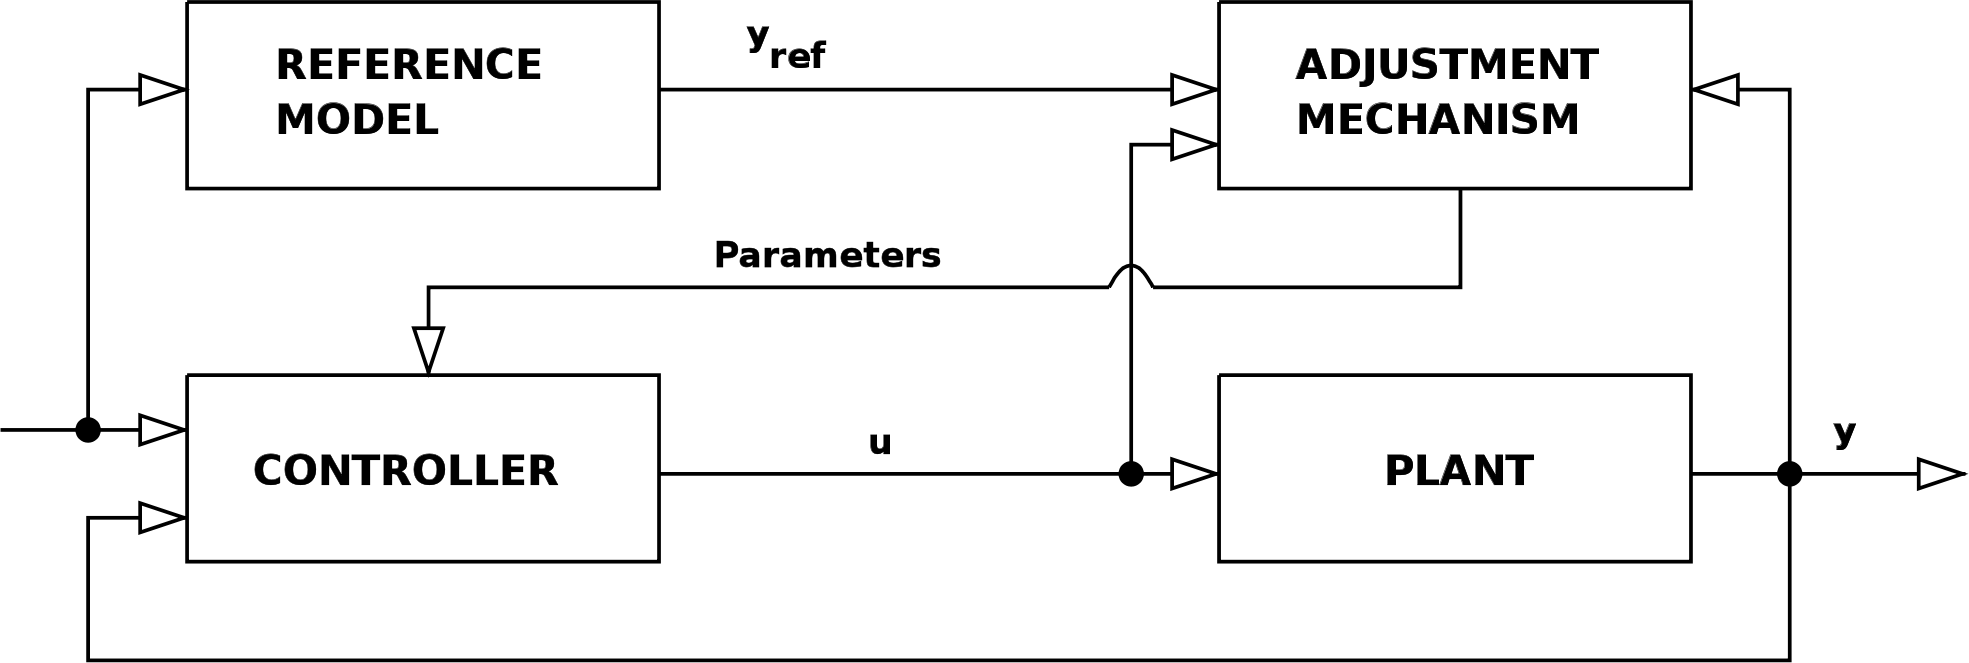
\includegraphics[width=0.8\textwidth]{fig/propostas/model_MRAC}
\caption{Modelo de um controlador adaptativo do tipo MRAC.}
\label{fig:cadapt}
\end{figure}

Utilizando o conceito básico deste tipo de controle e a reconfiguração dinâmica, é possível construir um controlador cuja forma é mudada segundo os requisitos dos sistema, i.e. hora seria um controlador proporcional, hora seria um controlador proporcional-integral-derivativo.
As dificuldades desta proposta dizem respeito implementa\c{c}\~ao de sistemas com reconfigura\c{c}\~ao dinâmica parcial e ao projeto do sistema que controlaria a troca entre controladores.

\subsection{Computação Genérica}
Um computador de computação genérica possui um conjunto fixo de instruções implementados em um sistema imutável no tempo.
A figura \ref{fig:mips} apresenta um processador MIPS de 5 estágios representando este um processador comum, i.e. imutável.
Os únicos elementos lógicos passíveis de alteração são as memórias.

\begin{figure}[h]
\centering
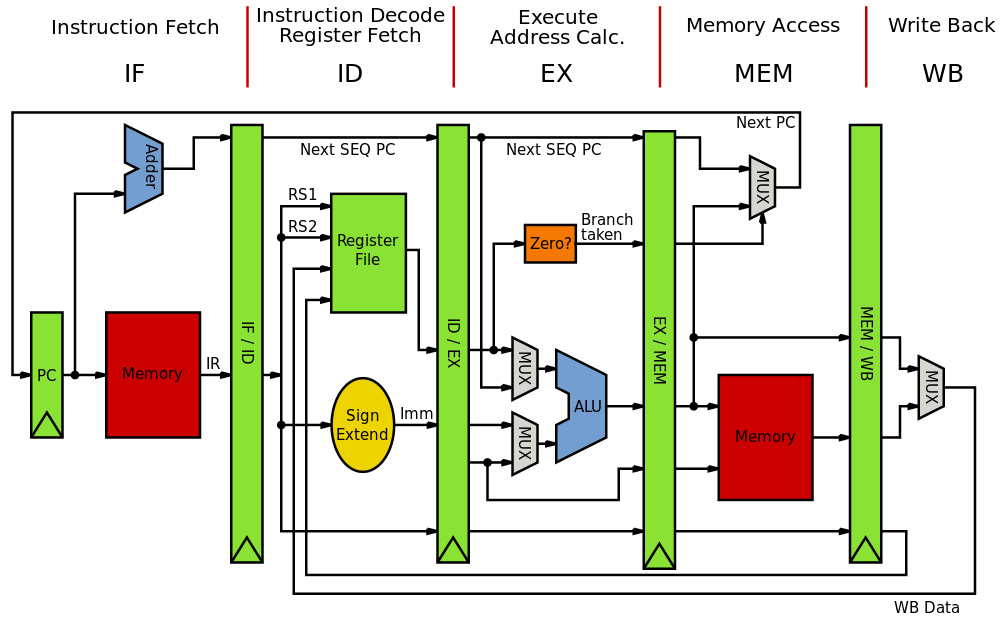
\includegraphics[width=0.8\textwidth]{fig/propostas/MIPS_Architecture_(Pipelined)}
\caption{Ilustração de um processador MIPS com \textit{pipeline} de 5 estágios.}
\label{fig:mips}
\end{figure}

O uso de autorreconfiguração este caso possibilitaria a redução do espaço físico necessário para a implementação de elementos da unidade de lógica e aritmética (ALU).
Esta modificação permitiria também uma diminuição no consumo de energia do processador, além de permitir que instruções de ponto flutuante fossem implementadas diretamente na ALU, sem a necessidade de extensão do processador.
Outra possibilidade é a implementação de um banco de registradores variável, permitindo ao compilador escolher quantos registradores utilizar em cada etapa do seu programa, otimizando ainda mais o desempenho deste.

As dificuldades deste projeto dizem respeito a necessidade de construção prévia de um processador genérico funcional e a inclusão de uma memória de configuração.
